\documentclass[letter,11pt]{article}
%\usepackage[round]{natbib}
\usepackage{setspace} 
\usepackage{dsfont}
\usepackage{amsfonts}
\usepackage{amsmath}
\usepackage{subcaption}
\usepackage{paralist}
%\usepackage{subfig}
\usepackage{times}
\usepackage{latexsym}
\usepackage{graphicx}
\usepackage[T1]{fontenc}
\usepackage{tikz}
\usepackage{url}
\usepackage{pgfplotstable}
\usepackage{titlesec}
\usepackage{color}
\usepackage{lipsum,adjustbox}
e\usepackage[font={small}]{caption}
\usetikzlibrary{positioning}
\usepackage{bbm}

\makeatletter
\newcommand{\@BIBLABEL}{\@emptybiblabel}
\newcommand{\@emptybiblabel}[1]{}
%\makeatother
\usepackage[hidelinks]{hyperref}


\usepackage{acl2012}
\graphicspath{{./plots/}}
\newcommand{\com}[1]{}
\newcommand{\oa}[1]{\footnote{\color{red}OA: #1}}
\newcommand{\lc}[1]{\footnote{\color{green}LC: #1}}

\begin{document}
	
\title{Conservatism and Over-conservatism in Grammatical Error Correction}

%\author{
%  Leshem Choshen\textsuperscript{1} and Omri Abend\textsuperscript{2} \\
%  \textsuperscript{1}School of Computer Science and Engineering,
%  \textsuperscript{2} Department of Cognitive Sciences \\
%  The Hebrew University of Jerusalem \\
%  \texttt{leshem.choshen@mail.huji.ac.il, oabend@cs.huji.ac.il}\\
%}


\maketitle

\begin{abstract}

\end{abstract}

\section{Introduction}

% Error correction 
% evaluation in error correction and its centrality
% faithfulness to the source meaning is important, and this has been noted but prev work, and evaluation is geared towards it
% gap in evaluation: however, steps taken to ensure conservativeness in fact push towards formal conservativism by their definition (theoretical claim about the measure)
% this may result in systems that make few changes. indeed we find that this is the case (empirical claim about systems)

% we pursue two approaches to overcome this bias.

% 1. increasing the number of references. this has been proposed before and pursued with m=2, but no assessment of its sufficiency or its added value over m=1 has been made. In order to address this gap we first charachterize the distribution of possible corrections for a sentence. We leverage this characterization to characterize the distribution of the scores as a function of $m$, and consequently assess the biases introduced by taking $m=1,2$ as with previous approaches. 
% We find that taking these values of $m$ drammatically under-estimate the system scores. 
% We back our analysis of these biases with an analysis of the variance of these estimators.
% We analyze the two commonly used scores, the M2 score often used for evalauted, and the accuracy score commonly used in training.

% 2. we note that in fact the important factor is semantic conservativism and explore means to directly assess how semantically conservative systems here through the use of semantic annotation. 
% We use the UCCA scheme as a test case, motivated by HUME.
% First question: is it well-defined on learner language. it is.
% Second question: are corrections in fact semantically conservate? to show that, we need to verify that the corrections make few (if any) semantic changes. our results indicate that this is the case: we show that the corrections are similar in (UCCA) structure to the source.

% conclusion (not in intro): we tried to use semantic similarity to improve systems.
% this is difficult due to semantic conservatism. we expect this will be in issue once evaluation is improved.
% future work.
% also future work: use multiple references in training (did people do that?)

% sections:
% 1. Introduction
% 2. Formal conservativism in GEC
% 3. First approach: Multiple References
% 3.1. A Distribution of Corrections
% 3.2. Scores (M2, accuracy index, accuracy exact)
% 3.3. Data
% 3.4. Bias of the Scores (setup + results)
% 3.5. Variance of the Scores (setup + results)
% 4. Second approach: Semantic Similarity
% 4.1. Semantic Annotation of Learner Language (prev work)
% 4.2. UCCA Scheme (see HUME)
% 4.3. Similarity Measures (including prev work of elior)
% 4.4. Empirical Validation: IAA, semantic conservativism vs. gold std
% 5. Conclusion

Grammatical Error Correction (GEC) is a challenging research field, which interfaces with many
other application areas of linguistics. The field is receiving considerable
interest recently, notably through the GEC-HOO \cite{dale2011helping,dale2012hoo} and
CoNLL shared tasks \cite{kao2013conll,ng2014conll}.
Within GEC, considerable effort has been placed on system evaluation,
which is notoriously difficult,
much due to the many valid corrections each source sentence may have
\cite{tetreault2008native,madnani2011they,chodorow2012problems,dahlmeier2012better}.\oa{why so many citations?}
%GEC evaluation is notoriously difficult, \lc{you left here a place for a cite, should I
%cite that this is difficult or reference to having many corrections}\oa{whatever best supports this claim}

An important criterion in the evaluation of GEC systems (henceforth, {\it correctors})
is their ability to generate corrections that are faithful to meaning of the source. In fact, many would prefer
a somewhat cumbersome or even an occasionally ungrammatical correction over a correction
that alters the meaning of the source \cite{brockett2006correcting}.
As a result, often when compiling gold standard corrections for the task,
annotators are instructed to be conservative in their corrections, e.g. in NUCLE \footnote{Daniel Dahlmeier, personal communication.} and the Treebank of LL \cite{nicholls2003cambridge}.
A recent attempt to formally capture this precision/recall asymmetry has
been the standardized use of $F_{.5}$ over $F_{1}$, where Precision is
emphasized over Recall \cite{dahlmeier2012better}.

However, favoring precision over recall may lead to reluctance of correctors to
make any changes (henceforth, {\it over-conservatism}).
Using a single reference correction, which is a common practice in GEC, compounds this problem,
as correctors are not only more severely penalized for making an incorrect change that for not making
any change, but are often penalized for making correct changes not found in the reference.

We present results that indicate that current state of the art systems suffers
from over-conservatism. Evaluating the output of all 15 systems that participated
in the recent CoNLL2014 shared task, we find that all of them
substantially under-predict corrections relative to the gold standard
(Section \ref{sec:formal_conservatism}). 

We pursue two approaches to address this gap, proposing
improved reference-based protocols to decrease the penalization of valid correction,
thereby avoiding over-conservatism.
First, we study the effect of increasing the amount of references,
which we denote by $M$ (Section \ref{sec:increase-reference}).
While previous evaluation explored the case of $M=2$,
no empirical assessment of its sufficiency or its added value over $M=1$
has been carried out.
%In our experiments we estimate the number of corrections necessary
%to cover the bulk of the distribution of possible corrections.
We consider two measures for
assessing the validity of a proposed correction relative to a set of references,
and characterize the distribution of their scores as a function of $M$.
Our findings suggest that using $M=1$ or $M=2$ dramatically under-estimates
the true performance of the systems, and commonly leads to cases where a valid
correction is more likely to be penalized than to be deemed valid
(Section \ref{sec:increase-reference}). 
We conclude with an analysis of
the statistical significance of these evaluation protocols.

Second, we pursue an alternative way of determining whether a correction faithfully
represents the semantics of the source, by measuring the
similarity of their semantic structures (Section \ref{sec:Semantics}).
%We define a measure, using the UCCA scheme \cite{abend2013universal} as a
%test case, motivated by its recent use for machine translation
%evaluation \cite{birch2016hume}.
In order to assess the feasibility of this approach, we annotate a
section of the NUCLE \cite{dahlmeier2013building}
parallel corpus. Our results support the feasibility of the proposed approach,
by showing that semantic structural annotation can be consistently applied
to learner's language (LL) and that the measure is less prone to undue penalization of
valid corrections.

The two approaches address the insufficiency of using too few references from
complementary angles. 
The first attempts to cover the bulk of the distribution of possible
corrections for a sentence, while the second
uses semantic instead of string similarity, in order to abstract away
from some of the formal variation between different valid corrections.

%%%%%%%%%%%%%%%%%%%%%%%%%%%%%%%%%%%%%%%%%%%%%%%%%%%%%%%%%%%%%%%%%%%%%%%%%%%%%%
\section{Over-Conservativism in GEC Systems}\label{sec:formal_conservatism}

%The field of GEC was always thriving for conservatism in its corrections, with the prominent example of using
%$F_{0.5}$ emphasizing precision over recall(\cite{ng2014conll}). we wish to highlight the problem that
%arises from pursuing this conservatism as done today.
%Then, we wished to be conservative, and we achieved that, why shouldn't we rejoice just yet? Theoretically, we might be progressing towards not correcting at all, instead of progressing towards correcting more accurately. 

%Manual analysis showed excessive formal conservatism and under correction.
%Albeit important, manual analysis is not enough and we aimed for generating some quantitative measures. 

We demonstrate that current correctors
suffer from over-conservatism: they tend to make too few changes to the source. 


\paragraph{Experimental Setup.}\label{par:experimental_setup}

Our experiments are on the NUCLE dataset,
a parallel corpus of LL essays and their corrected versions,
which is the de facto standard in GEC.
The corpus contains 1,414 essays in LL, each of about 500 words.

We evaluate all participating systems in the CoNLL 2014,
in addition to the best performing system on this dataset \cite{rozovskaya2014building}.
The particiapting systems and their abbreviations are: Adam Mickiewicz University (AMU),
University of Cambridge (CAMB), Columbia University and the University of Illinois at Urbana-Champaign (CUUI),
Indian Institute of Technology, Bombay (IITB), Instituto Politecnico Nacional (IPN),
National Tsing Hua University (NTHU), Peking University (PKU), Pohang University of Science and Technology (POST),
Research Institute for Artificial Intelligence, Romanian Academy (RAC), Shanghai Jiao Tong University (SJTU),
University of Franche-Comte (UFC), University of Macau (UMC),
Rozovskaya and Roth's best performing system (RoRo) \cite{rozovskaya2016grammatical}.
All are trained and tested on the NUCLE corpus.

We compare the prevalence of changes made to the source by the correctors, to the ones made by the NUCLE reference. In the evaluation, we discard all non-alphanumeric characters, both within tokens or as token of their own.

%In order to have better evaluation of the real goal of corrections we also
%compute all of the measures on ,
%based on the Cambridge First Certificate in English
%(FCE) \cite{yannakoudakis2011new},
%a new large parallel corpus containing only ungrammatical sentences of learners
%native of different languages.\oa{I didn't understand this sentence; how do we use this corpus?}


\paragraph{Measures of Conservatism.}
We consider three types of divergences between the source and the reference.

First, we measure to what extent \emph{words} were changed: altered, deleted or added.
To do so, we compute word alignment between the source and the reference, casting it
as a weighted bipartite matching problem, between the words of the source
and the correction. 
Edge weights are assigned to be the edit distance between the tokens.
\footnote{When breaking ties, we favor alignments where the place in the sentence is closer.}
We note that aligning words in GEC is much simpler than in machine translation,
as most of the words are kept unchanged, deleted fully, added, or changed slightly.
Following word alignment, we define the {\sc WordChange} measure
as the number of unaligned words and aligned words that are not the same.

Second, we quantify word \emph{order} differences by computing
Spearman's $\rho$ between the order of the words in the source sentence,
and the order of their corresponding words according to the word alignment considered above.
$\rho$ is closer to 0 where the word order is uncorrelated, and closer to 1 where they
exactly match. We report the average $\rho$ over all sentence pairs. 

Third, we report how many source sentences were split and how many concatenated by the references,
and by each of the correctors.


\begin{figure}[tbp]
  \centering
  \begin{subfigure}[]{0.4\textwidth}
  	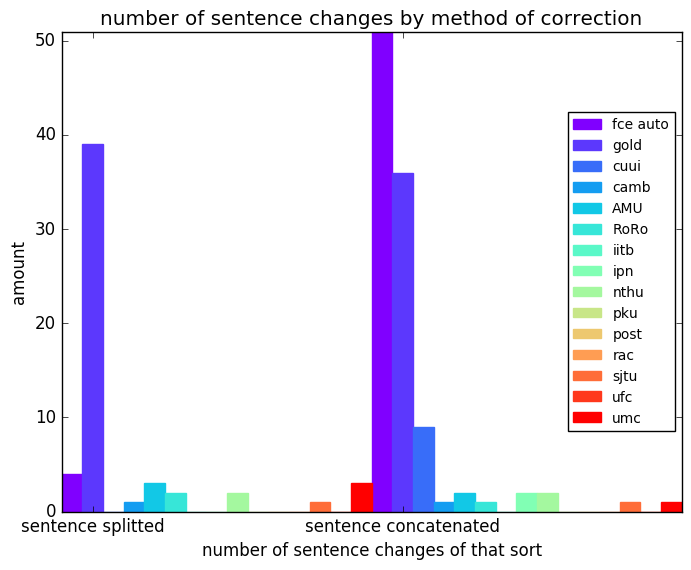
\includegraphics[width = \textwidth]{aligned}
  	\caption{Number of source sentences (y-axis) split 
  		(right bars) or concatenated (left bars) in the correction, according to the gold standard (striped column) and different correctors (colored columns). The gold standard makes about an order of magnitude more splits and concatenations than the correctors.\label{fig:split}}
  \end{subfigure}

  \begin{subfigure}[]{0.4\textwidth}
  	\com{\caption{\label{fig:rho}}}
    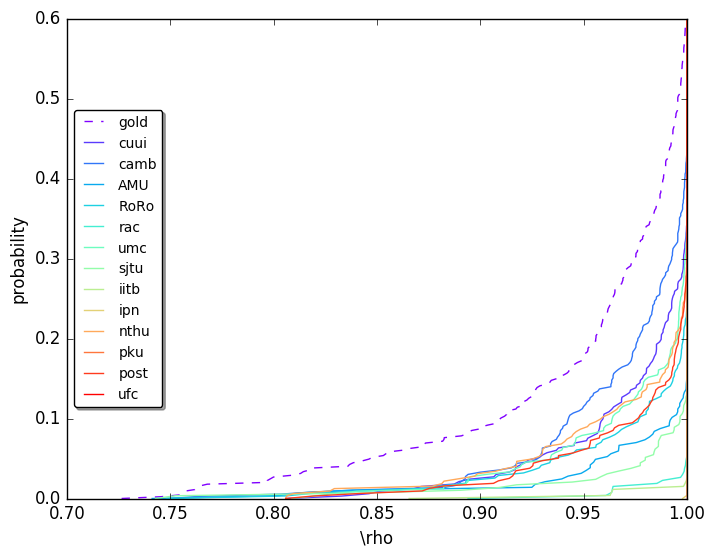
\includegraphics[width = \textwidth]{spearman_ecdf}
    \caption{Empirical cumulative probability (y-axis) of a sentence to get Spearman's rho values (x-axis) of word alignment. The gold standard(dotted line) makes word change alterations to more sentences than the correctors, and within these sentences, it changes order more substantially.\label{fig:rho}}
  \end{subfigure}

  \begin{subfigure}[]{0.4\textwidth}
  	%\caption{\label{fig:words_changed}}
  	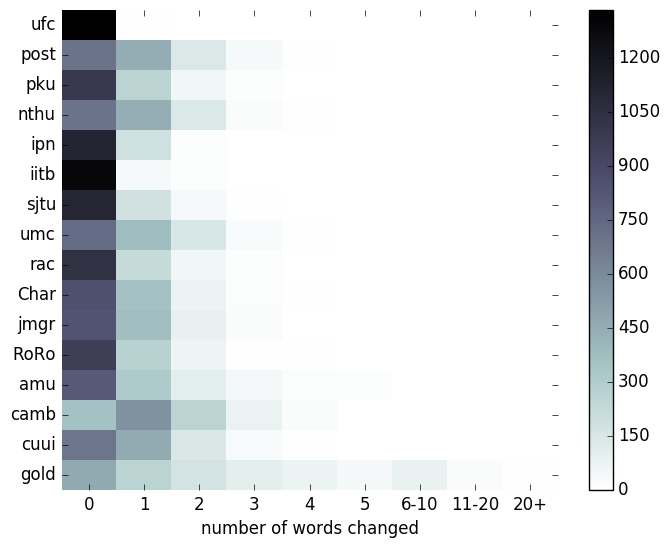
\includegraphics[width = \textwidth]{words_differences_heat}
  	\caption{Amount of sentences(heat) by number of words changed(x-axis) per system(y-label). The gold standard(bottom) corrects more words per sentences and more sentences relative to other systems.\label{fig:words_changed}}
  \end{subfigure}
  \com{\caption{(a) Number of source sentences (y-axis) split 
  		(right bars) or concatenated (left bars) in the correction, according to the gold standard (striped column) and different correctors (colored columns). The gold standard makes about an order of magnitude more splits and concatenations than the correctors.\\
  		(b) Empirical cumulative probability (y-axis) of a sentence to get Spearman's rho values (x-axis) of word alignment. The gold standard(dotted line) makes word change alterations to more sentences than the correctors, and within these sentences, it changes order more substantially.\\
  		(c) Amount of sentences(heat) by number of words changed(x-axis) per system(y-label). The gold standard(bottom) corrects more words per sentences and more sentences relative to other systems.\\
  		See \S\ref{par:experimental_setup} for a legend
  		of the systems.}\label{fig:over-conservatism}}
  \caption{\label{fig:over-conservatism}
    See \S\ref{par:experimental_setup} for a legend
    of the systems.}
  
  \com{
  	\begin{figure}[tbp]
  		\centering
  		\begin{subfigure}[]{0.4\textwidth}
  			\caption{\label{fig:split}}
  			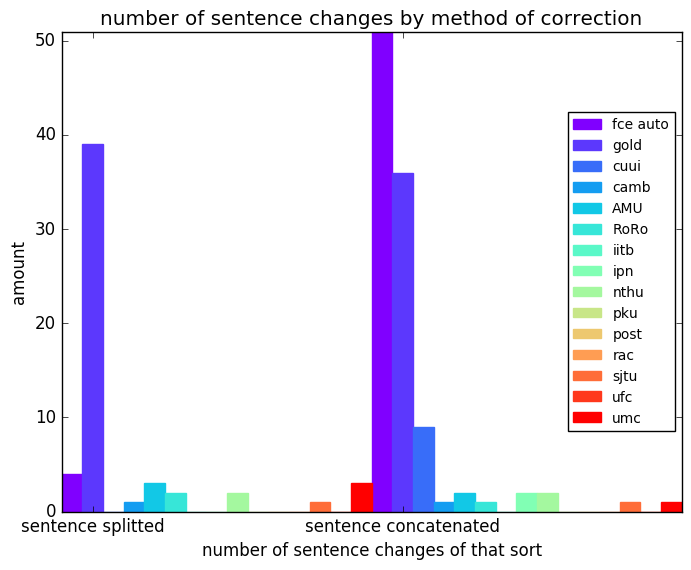
\includegraphics[width = \textwidth]{aligned}
  			\com{\caption{Number of source sentences (y-axis) split 
  					(right bars) or concatenated (left bars) in the correction, according to the gold standard (striped column) and different correctors (colored columns). The gold standard makes about an order of magnitude more splits and concatenations than the correctors.\label{fig:split}}}
  		\end{subfigure}
  		
  		\begin{subfigure}[]{0.4\textwidth}
  			\caption{\label{fig:rho}}
  			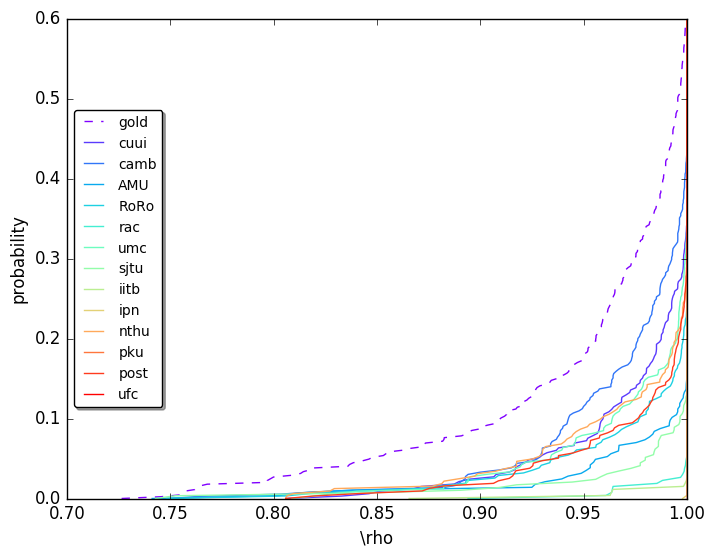
\includegraphics[width = \textwidth]{spearman_ecdf}
  			\com{\caption{Empirical cumulative probability (y-axis) of a sentence to get Spearman's rho values (x-axis) of word alignment. The gold standard(dotted line) makes word change alterations to more sentences than the correctors, and within these sentences, it changes order more substantially.\label{fig:rho}}}
  		\end{subfigure}
  		
  		\begin{subfigure}[]{0.4\textwidth}
  			\caption{\label{fig:words_changed}}
  			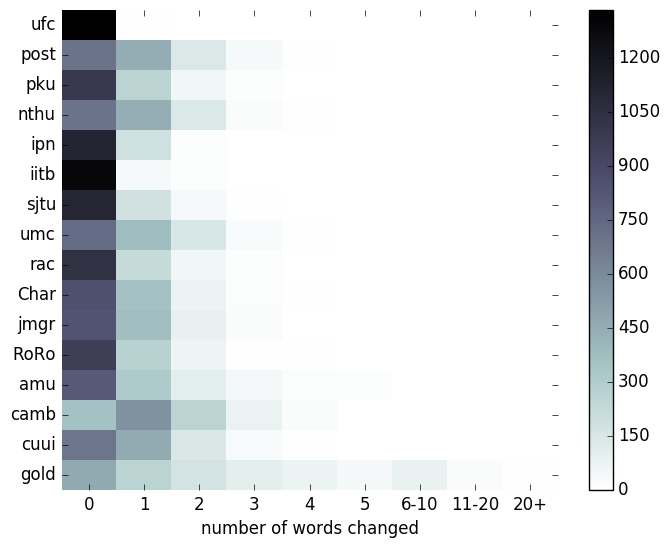
\includegraphics[width = \textwidth]{words_differences_heat}
  			\com{\caption{Amount of sentences(heat) by number of words changed(x-axis) per system(y-label). The gold standard(bottom) corrects more words per sentences and more sentences relative to other systems.\label{fig:words_changed}}}
  		\end{subfigure}
  		\caption{(a) Number of source sentences (y-axis) split 
  			(right bars) or concatenated (left bars) in the correction, according to the gold standard (striped column) and different correctors (colored columns). The gold standard makes about an order of magnitude more splits and concatenations than the correctors.
  			(b) Empirical cumulative probability (y-axis) of a sentence to get Spearman's rho values (x-axis) of word alignment. The gold standard(dotted line) makes word change alterations to more sentences than the correctors, and within these sentences, it changes order more substantially.
  			(c) Amount of sentences(heat) by number of words changed(x-axis) per system(y-label). The gold standard(bottom) corrects more words per sentences and more sentences relative to other systems.\\
  			See \S\ref{par:experimental_setup} for a legend
  			of the systems.\label{fig:over-conservatism}}
  		\com{\caption{	See \S\ref{par:experimental_setup} for a legend
  				of the systems. \label{fig:over-conservatism}}}
  	\end{figure}}
\end{figure}


\paragraph{Results.}
Figure \ref{fig:over-conservatism} presents the outcome of the three measures. 
%In \ref{fig:split} the amount of sentences each corrector has done is presented. In \ref{fig:words_changed} the accumulated sum of sentences by the words changed in each sentence of each of the correctors is presented. In \ref{fig:rho} the cumulative probability distribution of rho values out of all the sentences.
Results show that the reference corrections make changes to considerably more source sentences than any of the correctors, and within each changed sentence changes more words and makes more word order changes, often an order of magnitude more. For example, in the reference corrections there are 44 sentences which have 5 words corrections, where the most 5-word corrections by any corrector is 11.

For completeness, we also measured the prevalence of changes in
another corpus, the TreeBank of LL \cite[FCE]{yannakoudakis2011new}.
While $89.63\%$ of NUCLE sentences need corrections, FCE consists only of ungrammatical sentences. As expected, FCE is a bit less conservative than NUCLE by our measures.

%%%%%%%%%%%%%%%%%%%%%%%%%%%%%%%%%%%%%%%%%%%%%%%%%%%%%%%%%%%%%%%%%%%%%%%%%%%%%%%%%%%%%
		\section{Multi-Reference Measures}\label{sec:increase-reference}
		
		In this section we show that using commonly used number of references in reference-based evaluation yields a substantial under-estimation of system's performance. Specifically, our results indicate that using $M=1$ or $M=2$ leads to an under-estimation of the true performance of correctors by more than half.
		We discuss how such an under-estimation may lead systems to be overly conservative, and which values of $M$ may be more suitable for a reliable evaluation.
		
		%, 
		%While we still use string similarity measures, the use of multiple corrections captures
		%some of the variation in the possible corrections of a sentence.
		
		
		\subsection{Notation}
		
		We assume each source sentence $s$ has a set of valid corrections $Correct_s$,
		and a discrete distribution $\mathcal{D}_s$ over $Correct_s$ reflecting their prevalence.
		We will assume that $s$ is evaluated by
		$M$ independently sampled references from $\mathcal{D}_s$.
		
		Denote the set of source learner language sentences $X=x_{1}\ldots x_N \sim \mathcal{L}$, where
		$L$ is a distribution over all learner sentences from the domain. For each $x_i$, denote
		with $\mathcal{D}_{i}$ its distribution of corrections.
		%(i.e. a discrete distribution representing how many corrections are there and their relative frequency).
		Denote with $Y = \left\{y_{i}^{1},\ldots, y_{i}^{M}\right\} \sim \mathcal{D}_{i}$
		a sample of $M$ corrections.\footnote{Our analysis assumes $M$ is fixed across source sentences.
			Generalizing the analysis to sentence-dependent $M$ values is straightforward.}
		An assessment measure is a function which maps $C$ a correctors output or system, $X$ and $Y_1,\ldots,Y_N$ to
		a number in $[0,1]$. We use the term true measure when $y=Correct$.
		
		Define a corrector as a function from learner sentences to corrections.
		We assume this function is deterministic for simplicity of presentation,
		but our analysis holds for the case of a stochastic mapping as well.
		
		
		\subsection{Data}
		
		To be able to answer interesting statistical questions about assessment we first
		need to understand the behaviour of the distributions $D_x$. For that we sample
		52 sentences with a maximum length of 15 from the NUCLE test data
		. The restriction over the length was made to avoid having many different mistakes in the same text unit. It is reasonable to think corrections very far from each other are results of different mistakes, in that case we would not want the analysis to assess a very large number of corrections due to the exponential number of corrections when many unrelated mistakes occur.
		Sentences with less than 6 words were discarded, as they were mostly a result of sentence tokenization error,
		Histogram of sentence lengths showed a third of the mass is below this threshold.
		
		Albeit too expensive for assessment of each development cycle, human assessment
		by crowdsourcing is a very useful tool. Crowdsourcing assessment was shown to
		be helpful in different tasks such as translation
		\cite{zaidan2011crowdsourcing,post2012constructing}
		and in GEC \cite{madnani2011they}. % where the task is intuitive to non-experts.
		Thus, for each of the sentences gathered we asked Amazon Mechanical Turk workers to correct them, leading to 2600 corrections overall,
		50 per sentence. 4 sentences did not need correction according to a large part of the workers and hence were discarded.
		
		\subsection{Estimating The Distribution of Corrections}
		
		We begin by estimating $\mathcal{D}_s$ for each sentence, using the crowdsourced
		corrections. We estimated its distribution of corrections $\mathcal{D}_s$
		using {\sc UnseenEst} \cite{zou2015quantifying}, a non-parametric algorithm that
                estimates a multinomial distribution,
                in which only the individual values do not matter, only the distribution of probabilities
                across values.%\footnote{\href{https://github.com/borgr/unseenest}{UnseenEst}}
                The algorithm was originally developed for assessing how many
                variants a gene might have, including undiscovered ones.
                Thus, it is designed to estimate the distribution of variants that were not seen in the sample.
                Manual tests of unseenEst with small artificially created frequencies show
		satisfying results.\footnote{All data
		  we collected, along with the estimated distributions can be found in <to be disclosed
		  upon publication>}
		
		By the estimates from {\sc UnseenEst} most sentences have a large number of corrections with low probability accounting for a major part of the probability mass and a rather small number of frequent corrections. Specifically, the distributions tend to have steps with many corrections with the same (low) frequency. As example, a plot of three randomly selected sentences can be seen in \ref{fig:corrections_dist}. Considering variants with frequency more than $1\%$ to be frequent variants we calculated that on average there are 8.72 such variants which cover $52\%$ of the total probability mass.
		
		\begin{figure}
			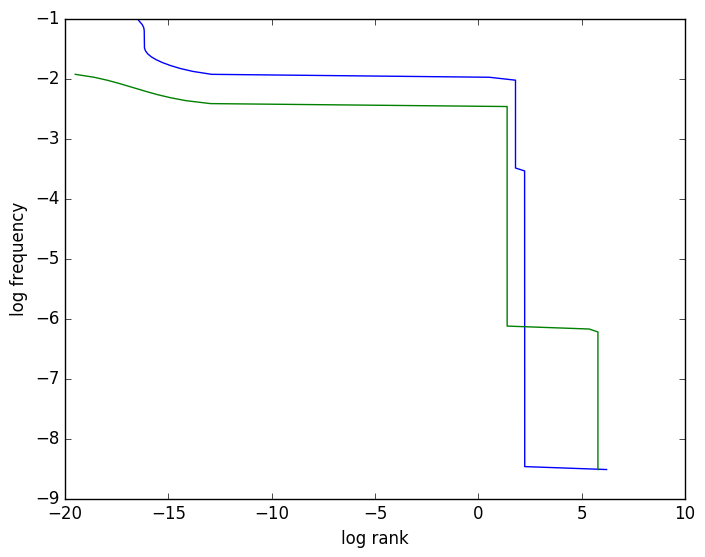
\includegraphics[width = 8cm]{exact_dists_plot}
			\caption{Frequency by rank of 2 corrections distribution. The distributions have steps containing many corrections that are just as probable with very low probability. 	\label{fig:corrections_dist}}
		\end{figure}
		
		\subsection{Assessment values} \label{subsec:Assessment-values}
		
		In the previous section we presented empirical assessment of the distribution of
		corrections to a sentence. We now turn to estimating the resulting bias, namely
                the under-estimation of reference-based similarity measures, for different values of $M$.
                %Our goal is to assess what value of $M$ would be a sweet spot,
                %which is both practical (as collecting references is costly) and reasonably
                %biased.\lc{do we indeed assess the sweet spot? we only show the door someone must walk through it according to the budget he has}
		
		We discuss two similarity measures. One is the sentence-level accuracy
                (also called ``Exact Match'') and the other is the GEC $F$-score.
		
		\paragraph{Sentence-level Accuracy.}
		Sentence-level accuracy is the number of sentences whose corrections
                exactly matches one of the references (also called ``Exact Match'').
                While this score is less
                commonly used than $F$-score as an evaluation
		measure of a corrector, it is a basic, interpretable measure and a variant of it was recently suggested as evaluation \cite{felice2015towards}\lc{added one evaluation method that helps our claim that accuracy is an interesting measure. should the other measure be cited somewhere?}. It is also
                closely related to the 0-1 loss function used for
		training statistical GEC systems
                \cite{chodorow2012problems,rozovskaya2013joint}. 
		
		Formally, given test sentences $X=\{x_1,\ldots,x_N\}$,
		their references $Y_1,\ldots,Y_N$, and a corrector $C$,
                we define $C$'s accuracy to be

		\begin{equation*}
		Acc(C;X,Y) = \frac{1}{N} \sum_{i=1}^n \mathds{1}_{C(x_i) \in Y_i}
		\end{equation*}

                Note that $C$'s accuracy is in fact an estimate of $C$'s probability to produce
                a valid correction for a sentence, or $C$'s {\it true accuracy}. Formally:

                \begin{equation*}
		  TrueAcc(C) = Pr_{x\sim{L}}\left(C\left(x\right)\in Correct_x\right)
		\end{equation*}
                
                %We estimate $C$s quality by sampling a set of source sentences
                %$x_1,\ldots,x_N \sim \mathcal{L}$, and evaluate the quality of $C(x_1),\ldots,C(x_N)$ relative
		%to the source. 

                The bias of $Acc(C;X,Y)$ for a sample of $N$ sentences, each paired with $M$ references
                is then

                \begin{small}
                \begin{align*}
                  TrueAcc(C) - \mathbb{E}_{X,Y}\left[Acc(C;X,Y)\right] = \\
                  TrueAcc(C) - Pr(C(x) \in Y) = \\
                  Pr(x \in Correct_x) \cdot \left(1 - Pr(C(x) \in Y \vert C(x) \in Correct_x) \right)     
                \end{align*}
                \end{small}
                  
		It is easy to see that the bias is not affected by $N$, only by $M$, and we therefore denote it
    with $b_M(C)$. As $M$ grows, $Y$ becomes a better approximation of $Correct_x$, and $b_M$ tends to 0.
		
		In order to gain insight about the evaluation measure and the GEC task
		(and not the idiosyncracies of specific systems), we consider an idealized learner,
		which is not biased towards a specific type of valid corrections. 
		Formally, we assume that $Pr(C(x) \in Y \vert C(x) \in Correct_x) = Pr(y \in Y)$, where $y \sim \mathcal{D}_x$.
		Under this assumption $b_M(C)$ can be written as the true accuracy of $C$ multiplied
		by a factor which is independent of $C$. We will hence assume that $C$ is perfect (i.e., its true
		accuracy is 1), noting that assuming any other value for $C$'s true accuracy would simply scale
		our graphs by that accuracy. Denote the bias of a perfect corrector with $b_M$. To recap:
		
		\begin{equation*}
		b_M = 1 - Pr_{x \sim L, Y \in \mathcal{D}_x^M, y \sim \mathcal{D}_x}(y \in Y)
		\end{equation*}
    
		We turn to estimating $b_M$ empirically. We note that $Acc(C;X,Y)$
		is a sum of Bernoulli variables (i.e., a Poisson Binomial distribution), 
		with probabilities $p_i = Pr_{y \sim \mathcal{D}_i}\left(y \in Y_i\right)$.
		
		Using the {\sc UnseenEst} estimations of $\mathcal{D}_i$, 
		we can estimate $p_i$ on our sentences, for any size of $Y_i$ (value of $M$). 
		However, as this computation is exponential in $M$, we estimate $p_i$ using
		sampling. Specifically, for every $M\in[20]$ and $i$ we sample $Y_i$ 1000 times, compute 
		the covered probability mass $Pr_{\mathcal{D}_i}[\{y: y \in Y_i\}]$ for each sample and 
		estimate $p_i$ to be their average. The resulting estimates for $p_i$ 
		define the estimate for the distribution of $Acc(C;X,Y)$.
		
		%Given a set of LL sentences $x_1,...,x_N$ and their corresponding references
		%$Y_1,...,Y_N$, we define the coverage of the reference set $Y_i$ for the sentence $x_i$ to be
		
		%\begin{equation*}
		%Cov\left(x_i,Y_i\right)=.
		%\end{equation*}
  
		%In order to gain insight into the accuracy measure, we need to know something about the distribution from which the given corrector chooses valid corrections. As each corrector might have its own biases, the most appealing choice would be to evaluate a corrector in which this distribution is the same as the one from which corrections for the gold standard are being drawn from. Formally, if $C\left(x_i\right) \in Correct_i$ then $C\left(x_i\right) \sim \mathcal{D}_i$. 
		
		%Thus, the second term in Equation \ref{eq:correction-in-gs} is $p_i = \mathbb{E}_{Y_i}[Cov(x_i,Y_i)]$. 
		%Therefore $Acc(C;X,Y)$ is distributed as
		%a Poisson Binomial random variable (divided by $N$), with probabilities $\{p_i \cdot CP\}_{i=1}^N$. \footnote{A Poisson Binomial random 
		%variable is a sum of Bernoulli variables with different success probabilities.} We also assume our corrector is always 
		%correct (so $CP=1$), but as noted earlier any other value for $CP$ would only scale the results by $CP$.
		
		\begin{figure}
			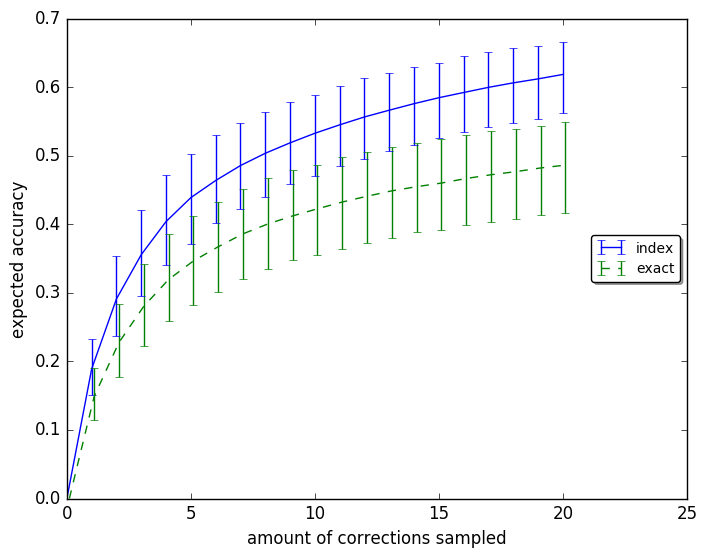
\includegraphics[width=8cm]{repeat_1000_accuracy}
			\caption{Mean accuracy values for perfect correctors with different number of references.} \label{fig:accuracy_vals}
		\end{figure}
		
		Figure \ref{fig:accuracy_vals} presents the expected values of $Acc(C;X,Y)$ according to our estimates of $p_i$ for
		different values of $M$. As our corrector is perfect, we would ideally expect its accuracy to be
		$Acc(C;X,Correct_i) = 1$. However, as the graph shows, even for values of $M$ which are much larger than
		those considered in the GEC literature (e.g., $M=20$), the expected accuracy is only of about 0.5.
		
		In order to examine whether our findings persist with a more relaxed measure, we examine the relaxed
		{\it Exact Index Match}, where two corrections $y$ and $y'$
		are equivalent relative to a source $x$ if in their alignments with $x$, $a$ and $a'$ respectively,
		if the number of deleted and added words is the same, and aligned words according to $a$ are
		changed (different from the aligned source word) if and only if, they are changed according to $a'$. Alignment is done in the same way as in \ref{sec:formal_conservatism}. Figure \ref{fig:accuracy_vals}
		shows that while expected accuracy is somewhat higher, still with $M=20$, it is no more than 0.65.
		
		To recap, we see that computing accuracy exactly requires many more references than was previously attempted.
		While common practice in GEC is to use $M=1$ or $M=2$, our simulations show that computing accuracy with
		so few references yields a scaling down of 5 or more. The graphs do show near linear behaviour from $M=9$ or
		so, which indicates that it reflects a reasonable balance between cost and bias.
		
		\paragraph{$F$-Score.}
		% present $F$-score
		% say that its analysis is more difficult
		% in order to estimate how different values of $M$ affect the bias of
		% the $F$-score, we use bootstrapping methods. again with a perfect corrector
		% explain briefly what we do.
		% show results
		% results are comparable to the index-based accuracy, i.e.,
		% an underestimation of the $F$-score
		% by a considerable factor for M=1,2, and they do not correspond to any natural point in the graph
		% near-linear behaviour with M=8, which is perhaps a practical solution
		While accuracy is popular as a loss function for training GEC systems,
		$F_\alpha$-score, the weighted harmonic mean of precision and recall, is standard when reporting a corrector's performance.
		
		Computing $F$-score for GEC is not at all straightforward. The score is computed
		in terms of matches of {\it edits}, which are sub-strings of the source
		that are replaced in the correction, and in the reference. Since correctors
		do not normally produce edits, $F$-score is defined optimistically, maximizing
		over all possible ways to annotate the source with edits, so as to end up with the correction. 
		The resulting optimization problem is NP-hard, but designated scorers
		have been developed to estimate it, notably the $M^2$ scorer 
		\cite{dahlmeier2012better}.
		
		Given the complexity of the definition of the measure, no analytical analysis is at hand (as with accuracy). Instead, we use a bootstrapping
		approach to estimate correctors' performance,
		incurred by the use of small values of $M$.
		In short, bootstrapping methods sample with repetition from the empirical distribution of the observed data to estimate properties (e.g. confidence-interval) of the statistic (e.g. $F$-score) over the distribution. 
		
		% how do we measure?
		To assess $F$ score we create a source text and $M$ gold standard texts based on the corrections we gathered.
		For each sentence which had at least one error according to the NUCLE gold standard we sample $M$ sentences uniformly from the
		gathered empirical data to replace it. We leave sentences that do not need corrections untouched. This results in reference texts accounting for the variability in different choices of corrections while approximating the reduction of variability of a big $N$ by consisting of $N$ sentences overall.
		We transform each gold sentence into a set of edits with a heuristic mapping based on the assumption aligned words that differ define an edit.\lc{this is not formal, on the other hand it is a total heuristic, no science is involved and not even a theory of how gold edits "should" look like. So what can people do with it? and we will probably not want to focus on yet another detail.}
		
		% what do we measure? we evalaute a perfect corrector
		As with accuracy, we assume the evaluated corrector is perfect and sample corrections for it
		(i.e., like a human, for every sentence $s$, it produces a correction in $Correct_s$),
		rather than the output of existing systems, both
		in order to avoid introducing any system-specific biases to the analysis,
		and the high cost of computing the true $F$-score of a system.
		
		% our results
		The results (see figure \ref{fig:F_Ms}) support the conclusions that there is an under estimation with $F_{0.5} = 0.42$ and an increase with bigger $M$ values.
		
		
		
		% discussion
		The effect of under estimation on evaluation and hence on how correctors are perceived is obvious. 
		Perhaps less obvious will be how under estimation affects the development
		process. We shall consider any evaluation which scores a wrong correction lower than no correction at all (e.g. $F$-score). For simplicity lets consider a scenario with only one sentence. We denote by $r>0$ the reward for a valid correction, $pu>0$ the punishment for a wrong correction and 0 otherwise. Thus, an average the score of a correction $x$ would be $S\left(x\right) = p\left(x\in y\right)*r - \left(1-p\left(x\in y\right)\right)*pu$.
		Under the assumption that development cycles or ML is gradually optimizing to get closer to the best solution, we will examine an all knowing perfect corrector.
		This corrector may take into account the probabilities of corrections to be in the gold standard. When choosing to correct such a corrector will choose the most frequent correction yielding $max_xS\left(x\right)$. Notably, not matter what are $r, pu$ when $p\left(x\in y\right)$ is small enough the perfect corrector will choose \emph{not} to correct.
		
		An interesting finding comes from the combination of the scores of a perfect corrector with the scores correctors get (with $M=2$). Some correctors get a result close to the perfect score, with one actually surpassing it. If we consider the results from section \ref{sec:formal_conservatism} it is evident that they are far from being a perfect corrector, as many sentences which evidently need correcting (even if there is more than one way to correct) are not corrected by them. Then how can they get such a high score?
		
		\com{\lc{Is that the right place for this general discussion of when can a system over-correct? Isn't that a prediction that drives us to look at the multi reference? I can't find any other place in which we discuss why over conservatism comes from this problem. could it be? where should this argument come?}
		Consider an all knowing perfect corrector, this corrector takes into account the evaluation coverage and knows the probabilities of corrections to be in the gold standard. Such a corrector will choose the most frequent correction, or no correction at all.  Notably, it will choose not correct when the increase in precision when the correction is in the gold standard contributes in expectation less to the $F$ score than the loss in recall for the times it is not in the gold standard.}
		
		One would like to suggest that the outstanding correctors have learned to correct like the specific annotator they have seen in the train. But as noted they do not correct enough, so that explanation lacks. An alternative explanation for it is that our prediction was right. The correctors avoid correcting sentences which they predict not to be well covered in the gold standard, gaining from that significantly.
		\lc{Supposedly why creating the gold standard texts and the edits is hard should come here. Not sure how important it is, well it is hard, but this is what we have chosen and I don't think of a specific criticism we should fend off by it.}
		%In respect to the edits, we note that the score for $M=2$ is a bit lower than one would expect\oa{why should I expect this?}. \lc{funny that you ask, well you did ask me that in person afterwards didn't you? :D}
		
		This would be a good place to mention the drawbacks and assumptions of the methods we are using, e.g. the explanation of a bad sampling is not probable but can not be refuted. We assume that the sentences we picked are a good representation of the overall sentences, but know they might be a bit simpler as we did not choose very long sentences for the reasons mentioned earlier. Another assumption is that the simple automatic edits are not a big shift in respect to the human edits.
		
		\com{This may result by the mechanical creation of edits. The different edits might give bias to the results\oa{but this is also true when evaluating real systems, no?}. Edit borders are not part of what correctors need to extract, in other words, it is an information that is not inherent to the task. Those edits are a disadvantage of the scoring system itself. It makes crowdsourcing much harder, and the edits are yet another thing that annotations often disagree upon(\cite{dahlmeier2012better}). It might be another reason that calls for use of another, more interpretable score.}
		\lc{as you have writen, edits bring bias to evaluation generally not only in our case, and they are actually not a part of the task, should we include this discussion somehow? we do talk about evaluation as the main frame of this discussion, this sounds to me like an interesting and important note}
		\lc{maybe the order of things in the discussion should change?}
		To conclude the main discussion of this section, if the NLP community has agreed one correction is not enough\cite{tetreault2008native}
		we can now say 2 is no magic number either. On both measures we see a large improvement in coverage when enlarging $M$, suggesting that a more reasonable $M$ to choose would be somewhere around 7 where the high probability corrections are probably covered and the graph turns semi-linear. The results also strongly support the hypothesis assessment values are very low, and hence might be a cause for over conservatism.
		Another conclusion to be made is that given a value from the assessment process we may estimate how low the value is in respect to the perfect assessment. Some may wish to correct for this under assessment.
		
		\subsection{On significance and variation}
		
		So far we have discussed the mean values of the assessment and showed they are lower bounds of the true value, and for the small $M$ in use a substantially under-estimate of it. However, since measures are often used as means of comparison between different systems, not less important than the bias is the variance of these estimators, and subsequently the significance level we may obtain with them. 
		
		\begin{figure}
			\includegraphics[width=8cm]{$F_{0.5}$_Ms_significance}
			\caption{F Score results with different sizes of gold standard.\label{fig:F_Ms}}
		\end{figure}
		\begin{figure}
			\includegraphics[width=8cm]{$F_{0.5}$_significance}
			\caption{F Score results for different correctors including confidence interval.\label{fig:F_correctors}}
		\end{figure}
		
		
		\paragraph{Accuracy:} As before, we start by considering the analytic formalism we have for accuracy. For that, sentences which were not corrected, or wrongly corrected have no variance with different $M$s, corrected sentences do. The variation of the Poisson binomial random variable we have is $\sum_{i=1}^{N}p_i\cdot\left(1-p_i\right)$ and as we divide the variable by $N$ we get $\frac{\sum_{i=1}^{N}p_i\cdot\left(1-p_i\right)}{N^2}$. 
		The variation is proportional to the number of sentences chosen given fixed $p_i$ values. Given a fixed $N$ variation gets lower as $p_i$s get away from $0.5$, a change that, from a certain point, occurs when $M$ is increased.
		
		\paragraph{$F$-score:} Analyzing variance of $F$ score is intractable\cite{yeh2000more}, thus, we use bias-corrected and accelerated bootstrap \cite{efron1987better}, to assess the $95\%$ confidence interval of different correctors with the current NUCLE test data ($M=2$), based on the same process as in \ref{subsec:Assessment-values}.
		
		We can learn from the results as seen in figure \ref{fig:F_correctors} what should be thought of as significant, for example the best performing corrector is significantly better than the second best we have checked, but is not significantly better than the other correctors proposed in the same article\cite{rozovskaya2016grammatical}. The results also  support the validity of the assessment method as the confidence interval indeed cover the actual scores seen in all of the cases. 
		
		The results in figure \ref{fig:F_Ms} suggest no great improvement of significance should be expected in the transition from $M=2$ to $M=5,8$.
		
		\subsection{Discussion}
		
		The factors controlling significance are two. Variation across sentences themselves (different $D_x$) which is reduced with $N$ and the variation across choices of corrections which might be reduced with either $M$ or $N$. One can rightly deduce that large $N$ is sufficient for variation, but it will not solve the other problems: under-estimation of true performance,
		over-conservatism, possible issues when training systems, and might be more costly than annotating a larger $M$ without acquiring more sentences and also annotating them.
		Choosing how to balance is dependent on the goals of the one collecting data, and affects over the mean value as well, as discussed in \ref{subsec:Assessment-values}. Thus, we bring supporting data and leave the decision to the reader. We just point out that such balancing questions have been studied in various fields such as genetics\cite{ionita2010optimal}.
		
		\com{\lc{I think this can be omitted}
			So, why is significance more complicated? Basically, because variance is more complex than mean. While $\mathbb{E}_{y\sim d_x, x\sim L}\left(\hat{S}\right)$ vary only as we change $M$
			the number of annotations, but not $N$ the number of corrections,
			$Var_{y\sim d_x, x\sim L}(\hat{S})$ depends on both. We try to assess and give an upper
			bound on how much it varies for different $M$ and $N$, allowing
			for both a smart allocation of resources when building a corpus and for assessing on given corpora whether two correctors are actually different.
		}
		

\section{Semantic Faithfulness Measure}\label{sec:Semantics}

%Conservatism is considered an important trait for a corrector, reflected for example
%in the selection of $F_{0.5}$, which emphasizes precision over recall, as the
%standard evaluation measure in GEC.
%In the previous section we followed the common approach in GEC evaluation and evaluated

%The thought that stands behind such emphasis is that a user
%would be understanding towards errors he did, of which he is probably
%not even aware, not being corrected, but would not be so understanding
%of corrections altering what he meant to say, in a way he perceives as wrong.

In this section we explore an alternative approach to overcoming the bias
introduced by the multitude of different valid corrections for an LL sentence, based
on semantic similarity.
The measure is based on the semantic similarity of the source and the proposed correction,
measured as graph similarity between their semantic representations.
We note that such a measure needs to be complemented with an additional
measure of fluency or grammaticality\cite{sakaguchi2016reassessing}, as it only captures
the faithfulness dimension, namely the extent to which
the meaning of the source is preserved in the correction.\lc{The reduction to semantic and error detection is another related way to convert this into an evaluation measure, one without references}

As a test case, we use UCCA to define the semantic structures \cite{abend2013universal}, motivated by
its recent use in semantic machine translation evaluation \cite{birch2016hume}.
We present results from two experiments that support the feasibility of the approach.
First, we show that semantic annotation can be consistently applied to LL,
through inter-annotator agreement(IAA) experiments.
Second, we show that a perfect corrector scores high on this measure, unlike on
the multi-reference measures disucssed in Section \ref{sec:increase-reference}.

%As semantic structures represent an abstraction over different realizations
%of a similar meaning,  In fact, $M$ plays no role in this approach, as the measure
%is defined not relative to a refernce but relative to the source sentence.

%as LL consists of many grammatical mistakes that makes syntactic
%analysis ill-defined for the task. We show evidence that this is the case, by having
%two annotators annotate a sub-corpus from the NUCLE dataset, and by measuring their
%inter-annotator agreement.
%%%Second, we ask whether corrections for a sentence indeed need to be faithful to the source. We seek to answer this question by measuring
%the semantic similarity between the source and the reference. We show support for an affirmative answer to this question 
%by annotating the references provided for the NUCLE dataset,
%and detecting high semantic similarity between the corresponding sentences on both sides. 

%\subsection{Background}

%Reliable assessment by a gold standard might be hard to obtain (see
%\ref{sec:increase-reference}), and human annotation for each output
%is great \cite{madnani2011they} but costly, especially considering the 
%development process. Under these conditions,
%%given a reliable semantic annotation we can enhance the reliability of our assessment. A simple way to do it is to somehow account in the assessment score for semantic changes. 
%Another, more ambitious way to do that might be to decouple the meaning
%from the structure. We propose a broad idea for a reduction from grammatical
%error detection and a comparable semantics annotation to grammatical
%error correction assessment. Lets assume we have both a reliable error
%detection tool and a good way to measure semantic changes. Then, we
%can transform assessment to a 3 steps assessment. 
%Step one, detect errors in the original text. Assess the amount of needed corrections, and the percentage of which that were changed.
%Step two, assess how much did the semantics change.
% Give a negative score for changing semantics.
%Last step, use
%the error detection again to assess how many errors exist in the correction
%output, whether uncorrected by the corrector or new errors presented
%by the correction process itself. 

%This assessment was partially inspired by the WAS evaluation scheme \cite{chodorow2012problems},
%in short it states we should account in the assessment for 5 types,
%not only the True\textbackslash{}False Positive\textbackslash{}Negative
%but also for the case where the annotation calls for a correction,
%and the corrector did a correction, but one that is unlike the annotation's
%one. With the proposed assessment we can measure how many of the corrections
%were corrected correctly (First + Second), and how many errors do
%we have eventually (Third) and combine them to get something similar
%to the Precision Recall that is widely used. We can also account for
%the places where the error was detected and check if it was corrected
%in a way that makes it grammatical and did not change semantics, the
%fifth type. We do that without getting a human to confirm this is
%indeed a correction.

%This system would be even more informative than the current one. Allowing assessment of
%what subtask exactly did the corrector fail to perform. Answering questions
%like: was the corrector too conservative and did not make enough corrections?
%Was it making changes in the right places but not correcting grammar successfully?
% as the corrector correcting grammar but changing things
%it was not supposed to? etc.

%Semantic structures were used for LL tasks \cite{king2013shallow}, but so far not to GEC. Some syntactic representations were suggested for this task, and as they are popular for structural representation we devote the next subsection to discuss them. Specifically we explain, why, apart from not being based on semantics, syntactic representation is not a good fit for LL and in particular not for enhancing the evaluation without enlarging reference number.

\subsection{Structural Representation in LL}

%The usefulness of syntactic parsing in NLP has encouraged a number of previous
%projects to define syntactic annotation for LL.
While linguistic theories propose that each learner
makes consistent use of syntax \cite{huebner1985system,tarone1983variability},
this use may not conform the syntax of the learned language, or of any other known
language. This entails difficulties in defining syntactic annotation for LL,
as, on the face of it, the language of each learner has to be annotated
in its own terms.

Existing approaches to syntactic representation of LL in NLP
differ in how they annotate syntactic errors.
\newcite{berzak2016universal} and \newcite{ragheb2012defining}
annotate syntactic structures according to the syntax used
by the learner, even if this use is not grammatical.
Such annotation may be unreliable as a source of semantic information,
as semantically similar sentences, formulated by different learners,
may have considerably different structures. \newcite{nagataphrase} take an opposite approach, and attempt
to be faithful to the syntax intended by the learner. However, such an
approach faces difficulties due to the multitude of different syntactic
structures that can be used to express a similar meaning.

%Syntactic representation is very popular and useful in many NLP tasks 
%\cite{mesfar2007named,ng2002improving,zollmann2006syntax}.
%Thus, one thought that comes to mind is to use grammar annotation 
%for LL.
%While not useless, grammatical approach is not well
%defined, and unclear both practically and theoretically.

In this section, we use semantic annotation to structurally
represent LL text. Semantic structures are faithful to the intended
meaning of the sentence, and not its formal realization, and thus face
less conflicts where the syntactic structure used diverges from
the one intended. We are not aware of any previous attempts to semantically
annotate LL text.


\paragraph{UCCA.}\label{sec:ucca}
UCCA is a a semantic annotation scheme, influenced
by typological and cognitive linguistic theories.
The scheme aims to provide a coarse-grained, cross-linguistically
applicable representation by directly reflecting the major semantic
phenomena represented in the text and abstracting away from
specific syntactic forms.

UCCA structures are directed acyclic graphs, where the words in the text 
correspond to (a sub-set of) their leaves.
The nodes of the graphs, called {\it units}, are either terminals or several elements jointly
viewed as a single entity according to some semantic or cognitive consideration.
The edges bear one or more categories, indicating the role of 
the sub-unit in the relation that the parent represents.

UCCA views the text as a collection of {\it Scenes} and relations between them.
A Scene, the most basic notion of this layer, describes a movement, 
an action or a state which is persistent in time.
Every Scene contains one main relation, 
zero or more {\it Participants}, 
which are interpreted in a broad sense, 
and include locations, destinations and complement clauses,
and {\it Adverbials}, such as manner or temporal descriptions.

Importantly, UCCA's categories directly reflect semantic, rather than distributional, distinctions .
For instance, UCCA is not sensitive to POS distinctions: a Scene's main relation can be a verb but also an adjective
(``He is {\bf thin}'') or a noun (``John's {\bf decision}'').
Indeed, \newcite{sulem2015conceptual} has found
that UCCA structures are preserved remarkably well across translations.

We use UCCA's standard annotation guidelines, without introducing any adaptations.

\subsection{Experimental Setup}

We employ two annotators, trained by annotating both LL and standard English
passages, until a high enough agreement was reached (6 hours of training in total).
Training passages were excluded from the evaluation.

We experiment on 7 essays and their corrections from NUCLE, each of about 400 tokens.
In order to measure inter-annotator agreement, we assigned 4 of these essays to both annotators
and compute their agreement (Section \ref{sec:iaa}).
In order to measure the faithfulness score for a perfect corrector, we annotate both
the source and corrected version for 6 essays, some of which were annotated by both annotators.

%For the different experiments 20 paragraphs were annotated, a table with the full
%information can be found in the appendix \ref{tab:annotated-paragraphs}.Overall, 2 LL
%and 2 corrected paragraphs were annotated by both annotators, 9 parallel paragraphs were
%annotated by the same annotator and 6 by different annotators.

%We see that as enough to be a proof that UCCA can be applied to LL, especially considering those numbers
%are a bit higher than the IAA originally reported
%for native English .
%We explain the rise in agreement by the fact that the guidelines and
%procedures were refined since UCCA was first introduced and not to
%superiority of UCCA for annotating LL. A similar F1
%score for IAA (0.849) over corrected paragraphs
%suggests the same.

%At least theoretically, semantics are well defined even on ungrammatical
%text. With the right tools we might capture at least some of the semantics
%of sentences and use them for the same purposes of grammatical annotation.
%In this work we will use Universal Conceptual Cognitive
%Annotation (UCCA)\cite{abend2013universal}, we will show that practically
%there are semantic annotation schemes that can be used for the purposes discussed.


\subsection{Semantic Similarity Measures}

\paragraph{Inter-annotator Agreement Measure.} We define a similarity measure over UCCA annotations 
$G_1$ and $G_2$ over the same set of leaves (tokens) $W$.
For a node $v$ in either graph, define its yield $yield(v) \subseteq W$ as its
set of leaf descendants.
Define a pair of edges $(v_1,u_1) \in G_1$ and $(v_2,u_2) \in G_2$ to be matching
if $yield(u_1) = yield(u_2)$ and they have the same label.
Labeled precision and recall are defined by dividing the number of matching edges
in $|G_1$ and $|G_2$ by $|E_1|$ and $|E_2|$. Their {\it DAG $F$-score} is their harmonic mean.
We note that the measure collapses to the common parsing $F$-score if $G_1$ and $G_2$ are trees.

\paragraph{Semantic Faithfulness Measure.} Computing a faithfulness
measure is slightly more involved, as the source sentence graph $G_s$ and its
correction $G_c$ do not share the same set of leaves.
\footnote{The use of graph kernels as a similarity measure between UCCA 
  structures is unsuitable here due to the small size of a UCCA DAG \cite{kashima2003marginalized}.} 

%Giving a more accurate
%measure than the upper bound suggested by \cite{sulem2015conceptual} for
%comparing two parallel texts in different languages, while keeping
%the essence of comparing how many of the aligned nodes conserve meaning and tag. For that we may think for a moment on GEC as
%translation from LL to Proper English, and a good translation
%would be a translation which keeps the meaning but has the syntax
%of English. Considering that, just like in translation, we can align words from the LL to the corresponding words in English
%and keep record of how many of those nodes kept their labels.

%As comparing labels is trivial, and done before us. We should focus on how we propose to align nodes. 
%First, note that comparison should not be at
%the token level, as we want to allow tokens to be corrected - replaced or removed -
%as long as the higher structures convey the same meaning. We thus
%prune the labels above the leaves, the tokens of the sentence. To
%define an alignment of the nodes, we suggest some possible ways, all
%based on first aligning the words in order to give order to the DAG and then comparing the structure in one way or another.

We assume a (possibly partial, possibly many-to-1) alignment between $G_s$ and $G_c$,
$A \subset V_s \times V_c$. An edge $(v_1,v_2) \in E_c$ is said to match an edge
$(u_1,u_2) \in E_s$ if they have the same label and $(v_2,u_2) \in A$. Recall (Precision)
is defined as the ratio of edges in $E_s$ ($E_c$) that have a match in $E_c$ ($E_s$) respectively, and
$F$-score is their harmonic mean. We note that this measure indeed collapses to the
DAG $F$-score discussed above where $A$ includes all pairs of nodes in $E_s$ and $E_c$ that have
the same yield.

In order to define the alignment between $V_s$ and $V_c$, we begin by aligning the leaves
(tokens) in $V_s$ and $V_c$ using the same method detailed in Section \ref{sec:formal_conservatism}.
Denote the results leaf alignment with $A_l \subset Leaves_s \times Leaves_c$.

We cast the problem of finding a node alignment as a maximum weighted bipartite matching problem between
the set of nodes $V_s$ and the set $V_c$, where the weight of an edge $(u,v) \in V_s \times V_c$ is
defined to be $w(u,v) = \frac{\vert A_l \cap (yield(u) \times yield(v))\vert}{\vert yield(u) \vert} $.
$A$ is defined to be the maximum weighted matching, excluding edges
with weight 0.\oa{why do we use many-to-1? {\bf this doesn't make sense because it favors
nodes up the tree. better to normalize}}
The resulting $F$-score measure, using this computation of $A$ is called {\sc UCCASim}.

We note that 
{\sc UCCASim} is somewhat more relaxed than DAG $F$-score defined above,
as it aligns two nodes not only if their yields are in perfect alignment with
one another, but it may also match nodes whose yields are in partial alignment
with one another. This relaxation is necessary given that a correction often adds
or removes nodes, thus eliminating the possibility of a perfect alignment between
the sentences. 

%Then for each node in $v \in V_s$, we compute its descendent leaves $yield(v) \subset Leaves_s$ as before,
%and compute their projection $yield'(v) = \{u \in Leaves_c:(v,u) \in A_l\}$.
%We now define the node alignment to be $A = \{(u,v) \in V_s \times V_c : yield'(u) = yield(v) \}$.
%We note that $A_l \subset A$ and that if $V_s$ and $V_c$ share the same tokens,
%this computation again reduces to DAG $F$-score.

While generalizing DAG $F$-score, this approach has the shortcoming
of being asymmetrical. We therefore report both the resulting $F$-score when aligning
from the source to the correction and the other way around.\oa{this paragraph will not be
  true if we do 1-1 alignment}

For completeness, we also replicated the protocol of \newcite{sulem2015conceptual},
which we call {\sc DistSim}.
For a given UCCA label $l$, denote $c_i(l)$ the number of $l$-labled UCCA nodes
in the i-th source sentence, and $d_i(l)$ the number of $l$-labled UCCA nodes
in its corresponding correction. We define {\sc DistSim}(l) between these
sentences to be $\frac{1}{N}\sum_{i=1}^N \vert c_i(l) - d_i(l) \vert$, where
$N$ is the total number of sentence pairs.

%A first and most straightforward approach would be to compare all
%pairs of nodes in parallel paragraphs and to each node from one paragraph
%assign the one most similar node, span wise from the other. That approach
%is quite similar to the IAA aligning, but it
%has three drawbacks; it is asymmetric; it may be over optimistic aligning
%nodes without considering the DAG structure; and it might be
%slow for many nodes. Being asymmetric is not much of a problem. If we thrive for symmetry
%we can compute the measure twice and use the results mean,
%that would also be the case for other asymmetric methods we suggest.
%In order to address the other drawbacks we propose different aligning methods.

%A second method driven by the assumption that nodes higher in the
%hierarchy are more important to the semantic representation is measuring
%the largest cut in which nodes are aligned (top down) to each other
%and have the same labels. This is a harsher lower similarity
%score but one of which might be more representative of the semantics
%that are kept and hopefully more informative for tasks that will use it.

%A third type of methods were token similarity methods, these methods
%use one kind of aligning (top down, bottom up or pairwise) and only
%compare the meaningful nodes. This was called upon by \cite{sulem2015conceptual}. 
%This approach makes sense due to the fact that some labels
%are well defined and thought upon while others are still vague and
%call for future work on refining or adjusting them, moreover, some
%labels are more semantic while other labels are currently just a place
%holder as each node must get a level, and the semantic role is not
%always clearly defined (e.g., the word ``is'' in ``he is walking''
%seem to be more syntactically related than semantically. In UCCA it is tagged as a \textit{function} word.). The unused
%labels are center, elaborator, function, relation, linker, ground
%and connector.

%A bit different way than all the others is to compute the labeled
%tree edit distance\cite{zhang1989simple}, for that we first needed
%the trees to be ordered, we did that in a top down fashion. An interesting
%future work would be to use unordered tree edit distance methods\cite{zhang1992editing}.

%We see that measurements for symmetry that are similar to the inter
%annotator agreement measure also suggest high stability, achieving
%scores not much lower than the one different annotators get for the
%same paragraph. This result is quite strong as an inter annotator
%agreement is the upper bound being the score of comparing a paragraph to itself. 
%Most importantly we learn from it all that even when correcting grammatical errors,
%the semantic structure (as represented by UCCA at least) is hardly changed and thus
%can be used as a tool to avoid introducing semantic changes when trying to only change grammar. 
%The symmetry measures we introduce can be used to enforce semantic conservatism.
%In conclusion, we have shown some direct ways to measure
%semantic faithfulness. Such ways will allow correctors to be less formally conservative
%while controlling semantic conservatism. Thus, focusing on what users - and hence we - are more interested in.


\subsection{The Faithfulness of a Perfect Corrector}

We obtain an IAA DAG $F$-score of 0.845
(Precision 0.834, Recall 0.857), which
is comparable to the IAA reported for English Wikipedia texts by \cite{abend2013universal}.
As another point of comparison, we doubly annotated 3 corrected NUCLE passages, obtaining a similar agreement rate.

These results suggest that annotating LL with UCCA does not lead to any degradation of IAA, and can be applied as consistently to LL text as to non-LL texts.

Table \ref{tab:Distances} on its left presents the {\sc UCCASim} scores obtained by comparing the NUCLE gold standard and the source sentences, or equivalently the {\sc UCCASim} score of a perfect corrector.
In order to control for differences between the annotators, we explore both
a setting where the two annotations were annotated by the same annotator,
and settings where they were annotated by different annotators.
In order to obtain an upper bound on the {\sc UCCASim} of a perfect corrector,
the table also presents {\sc UCCASim} scores between 
source sentences annotated by
different annotators.

Our results indicate that a perfect corrector receives a faithfulness score comparable
to the IAA, which is an indication that {\sc UCCASim} is indeed
insensitive to the surface divergence between a source sentence and its valid correction.
However, more work is required to establish whether the converse holds, namely that the measure is sensitive
to unfaithfulness of a proposed correction.
This, of course, depends on the scope of distinctions covered by the semantic annotation.
In UCCA's case, it is argument structure, the connections between scenes etc.

Our attempts to conduct experiments to determine {\sc UCCASim}'s sensitivity to erroneous
corrections introduced by the correctors described in Section \ref{sec:formal_conservatism} were
unsuccessful, as there are only very few cases of structural (rather than word-level)
corrections which these systems make (see Figure \ref{fig:over-conservatism}).
We expect that once the over-conservatism of existing correctors is resolved,
such an evaluation will be made possible.

%Finally, we present as a control measure and a bound on the best score
%we can expect to get in such comparison the scores of paragraphs
%in which we compare two annotations for the same paragraph using all
%the similarity measures discussed, it can be thought of as a different
%way to defining IAA. Note that a similarity
%of 1 and distance of 0 is indeed reached when comparing an annotation with itself.

Finally, The right-hand side of Table \ref{tab:Distances} presents {\sc DistSim} between the source and reference sentences.
Our results are similar to the ones obtained by \newcite{sulem2015conceptual},
who compared standard English sentences and their French translations.


\begin{table}[h!]
  \centering
  \singlespacing
  \begin{tabular}{c|c|c|c||c|c|}
  	\cline{2-6} 
  	& \multicolumn{3}{c||}{\sc UCCASim} & \multicolumn{2}{c|}{\sc DistSim}\\ \cline{2-6}
  	& s$\rightarrow$r & r$\rightarrow$s & avg & A+D & Scene\
    \\
    \hline
    Same & 0.92 & 0.91 & 0.92 & 0.97 & 0.96
    \\
    Different & 0.85 & 0.83 & 0.84 & 0.96
    & 0.93
    \\
    Baseline & 0.85 & 0.81 & 0.83 & 0.95 & 0.96
	  \end{tabular}
  \caption{Similarity measures for different mapping, their average and token analysis. For {\sc UCCASim} the baseline is the score over two LL annotations and for {\sc DistSim} the translation between English and French. For mapping the baseline one annotator was consistently considered the reference and the other the source. The correction similarity introduces less noise than the different annotators and annotating LL changes even less than translating does.\label{tab:Distances}}
\end{table}


%%%%%%%%%%%%%%%%%%%%%%%%%%%%%%%%%%%%%%%%%%%%%%%%%%%%%%%%%%%%%%%%%%%%
\section{Conclusion}

We presented results that indicate that state of the art systems in GEC suffer from over-conservatism. We hypothesize that this over-conservatism results from the use of scoring functions that not only tend to more severely penalize introducing grammatical errors, than to overlooking existing ones, but also to often penalize systems for generating valid corrections, if these are not included in the set of references.
In fact, in many cases systems are more likely to be penalized for the generation of
a valid correction than to receive credit for it, due to the small number of references
taken into account.

We explored two approaches for tackling this caveat in current measures, one by
increasing the number of references, and the other by employing a semantic similarity
measure for estimating the semantic faithfulness of the correction to the source.
We compute the scores a perfect corrector would receive with both approaches, showing that both increasing the number of references and using semantics are less prone to severely penalize valid corrections, and thus constitute valid solutions for addressing this caveat.

In many of the uses for correction, the user does know his grammar is not perfect and would accept a change in grammar when needed.
Because of this approval we also hypothesis, and it may call for a user study to prove or disprove this hypothesis, that users might accept a correct text unit of theirs being corrected to another correct text unit with the same meaning.
This would be an example of being faithful but not conservative.
Maybe even more importantly, we aim to have as many correct sentences as possible, but as neither the grammar is fully correct in the first place, nor is the user's understanding of it, failing to correct grammar is acceptable. Changing meaning will be totally unacceptable, and also surely detectable by the user. In other words, the users do expect the corrector to be active and not too conservative, but only as long as it is faithful. 

Moreover, as correctors are based on statistics, they might even
just correct to a more common way of saying the same thing. Such unnecessary
correction is not conservative, and at GEC maybe be unwanted, but not strictly unwanted as overall
it is still faithful. Additionally, some may even
consider such correction a needed one because it has a better grammar considering
Fuzzy Grammar\cite{lakoff1973fuzzy,madnani2011they} or a more fluent
way to say the exact same thing. The latter was recently suggested as a necessary
shift in the goals of GEC\cite{sakaguchi2016reassessing}.
Considering all this, we propose that next generation correctors and evaluation will be focused on faithfulness
when possible rather than on conservatism. Of course that with the evaluation comes the development
and it all suggests that it might be beneficial to incorporate faithfulness not only for assessment
but also as a feature for correctors. 



\bibliographystyle{acl2012}
\bibliography{propose}

\com{
\appendix
\section{Annotated paragraphs}
\begin{table}[]
	\centering
	\begin{tabular}{lll}
		Annotator-id & NUCLE-id & type      \\
		1         & 2  & corrected \\
		2         & 2  & corrected \\
		1         & 2  & learner   \\
		2         & 2  & learner   \\
		1         & 3  & corrected \\
		2         & 3  & corrected \\
		1         & 3  & learner   \\
		2         & 3  & learner   \\
		1         & 5  & corrected \\
		2         & 5  & corrected \\
		1         & 5  & learner   \\
		2         & 5  & learner   \\
		1         & 6  & learner   \\
		2         & 6  & learner   \\
		2         & 7  & corrected \\
		2         & 7  & learner   \\
		1         & 8  & corrected \\
		1         & 8  & learner   \\
		1         & 10 & corrected \\
		1         & 10 & learner  
	\end{tabular}
	\caption{The list of paragraphs annotated, showing which annotator annotated it, which type of language is used in it and the corresponding id in the NUCLE corpus. Note that parallel paragraphs have the same id.\label{tab:annotated-paragraphs}}
\end{table}
}

\end{document}


